% !TEX root = ../main_sys.tex
%
\chapter{Quality Assurance}
\label{sec:quality_assurance}

In this chapter we describe our continuous integration pipeline, the testing strategy, our git strategy and our documentation strategy that are used during development of the ML4PdM library.

\section{Continuous Integration}
\vspace*{-10mm}\hfill{\fontfamily{phv}\normalsize\emph{Christopher Zinda}}
\label{sec:quality_assurance:ci}

For continuous integration while developing the ML4PdM library, the GitLab CI/CD pipeline is used. It is executed on every commit to the master and develop branches as well as merge requests and tags. This ensures a sufficient quality control while limiting the number of failed pipelines by not including feature branches.

The CI/CD pipeline contains two jobs which are running in parallel. One job submits the changes to the SonarQube\footnote{\href{https://www.sonarqube.org/}{https://www.sonarqube.org/}} which is a self-hosted version of the SonarCloud\footnote{\href{https://sonarcloud.io/}{https://sonarcloud.io/}}. It will detect bugs, vulnerabilities, code smells, failed tests and test coverage in an automated manner. The results are displayed on a detailed dashboard for manual analysis by the developers. The second job will use the Sphinx\footnote{\href{https://www.sphinx-doc.org/en/master/index.html}{https://www.sphinx-doc.org/en/master/index.html}} Python documentation generator to automatically generate a static HTML page as well as a PDF document containing the class documentation and usage examples. The documentation is described in detail in section \ref{sec:quality_assurance:doc}.

A failed pipeline execution has to be fixed by the author of the changes. Merges to the master branch are not allowed until all errors have been corrected and the pipeline runs without errors. This will always ensure a tested and working code base on the master branch.
\newpage
\section{Testing Strategy}
\vspace*{-10mm}\hfill{\fontfamily{phv}\normalsize\emph{Paul Fährmann}}
\label{sec:quality_assurance:testing}

We will use \textit{pytest}\footnote{\href{https://docs.pytest.org/en/stable/}{https://docs.pytest.org/en/stable/}} for our automated tests. We will try to automate all our tests, but we probably will have tests that are more sophisticated and it's unsure if they can be automated. We can identify three levels of testing which are progressively harder to test automatically:
\begin{enumerate}
	\item Unit Test\\
	      We test individual functions and classes.
	      \begin{itemize}
		      \item Testing all parser classes and their configuration classes as well as the DataSet class.\\
		            Testing some example configuration files, in wrong and correct format. Also using different sensor data types and testing the functionality of \verb|@Target| in our data format.
		      \item Testing every pipeline element class.\\
		            Checking that the input and output format types are correct and also that the classes calculate what they should calculate according to our topic study and system design document.
		      \item Testing the Evaluator\\
		            Checking that the evaluator correctly loops through all the components and that it aggregates the resulting scores/losses correctly.
		      \item Testing the metrics\\
		            Testing that the metrics calculate the correct values.
	      \end{itemize}
	\item Integration Test\\
	      Testing that our predictor/transformer classes can work together with the sklearn classes in make\_pipeline and make\_union as well as other ways of integrating \verb|sklearn| and \verb|ml4pdm|.
	\item System Test\\
	      For three different knowledge-levels of users (beginner, intermediate, professional) we have tests of our system.
	      \begin{enumerate}
		      \item[1)] Beginner level: check that our library/evaluator can be used easily via the command line and get out error/score values and an actual model.
		      \item[2)] Intermediate level: check that a small part of predefined pipeline can be changed easily.
		      \item[3)] Professional level: check that each component of our library can be accessed and used individually without changing anything in the library itself.
	      \end{enumerate}
\end{enumerate}

\section{Documentation Strategy}
\vspace*{-10mm}\hfill{\fontfamily{phv}\normalsize\emph{Vinay Kaundinya}}
\label{sec:quality_assurance:doc}

Here we present a wholesome strategy for documenting code in describing its use and functionality to users, that is applied in the development of ML4PdM approaches. The idea is to keep it concise enough to be easy to maintain but still be elaborate enough for users to understand how to use the documented code.

\subsection{Documenting Code}
We use \textit{Docstrings} in documenting our code. Docstrings are built-in strings when configured correctly can help in documenting library's functionality for its users.

Docstrings have documentation of code written within triple-double($"""$) quotes.
\begin{figure}[H]
	\centering
	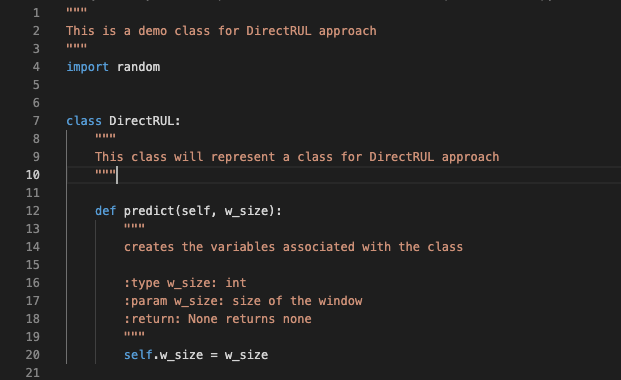
\includegraphics[width=10cm,height=6cm]{gfx/ex_docstring.png}
	\caption{Docstrings used in demo code describing a classes and its methods and parameters.}
	\label{fig:docstring}
\end{figure}
Docstrings are created for classes, as well as any class methods. The docstrings are placed immediately following the class or class method declaration. A docstring for a class should contain the following mandatory points,
\begin{itemize}
	\item A brief summary of its purpose and behavior.
	\item Any public methods, along with a brief description.
	\item Any class attributes.
\end{itemize}
An example of the same is also shown in the figure \ref{fig:docstring}.

\subsection{Document Generation}

We use Sphinx to generate documentation from docstrings in the python scripts of the project. Sphinx can provide documentation output in HTML, LaTeX (for printable PDF versions), ePub, Texinfo, manual pages, plain text formats. Sphinx uses reStructuredText as its markup language, and many of its strengths come from the power and straightforwardness of reStructuredText.

A reStructuredText document is made up of body or block-level elements, and may be structured into sections. Sections are indicated through title style (underlines and optional overlines). Sections contain body elements and/or subsections. Some body elements contain further elements, such as lists containing list items, which in turn may contain paragraphs and other body elements. Others, such as paragraphs, contain text.

Sections are identified through their titles, which are marked up with adornment: "underlines" below the title text, or underlines and matching "overlines" above the title.
Below are examples of section title styles:\begin{verbatim}
===============
 Section Title
===============

---------------
Section Title
---------------

Section Title
=============

Section Title
-------------

Section Title
`````````````

Section Title
*************

Section Title
+++++++++++++\end{verbatim}
\begin{figure}[H]
	\centering
	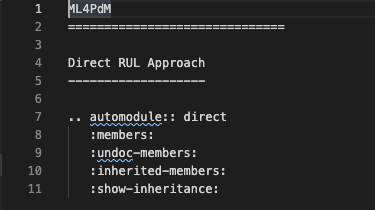
\includegraphics[width = 6cm]{gfx/ex_rst.png}
	\captionsetup{justification=centering}
	\caption{Example of reStructuredText document.}
	\label{fig:rst}
\end{figure}
In our document we use \textit{sphinx\_rtd\_theme} theme and this is configured while installing the sphinx document generator.
The documentation is then structured into following sections:
\begin{itemize}
	\item \textbf{Installation}: In this section we describe ways to invoke this library and all the other installation details.
	\item \textbf{Examples}: Here we list some examples of how the ML4PdM library can be used.
	\item \textbf{ML4PdM}: All the ML4PdM approaches, along with their classes, methods and parameters are documented under this section.
	\item \textbf{Release}: This section lists all the releases.
	\item \textbf{Glossary}: This section consists of keyword definitions used in documenting the approaches.
	\item \textbf{References}: Lists all the references to scientific papers, websites, books and datasets.
\end{itemize}
\begin{figure}[H]
	\centering
	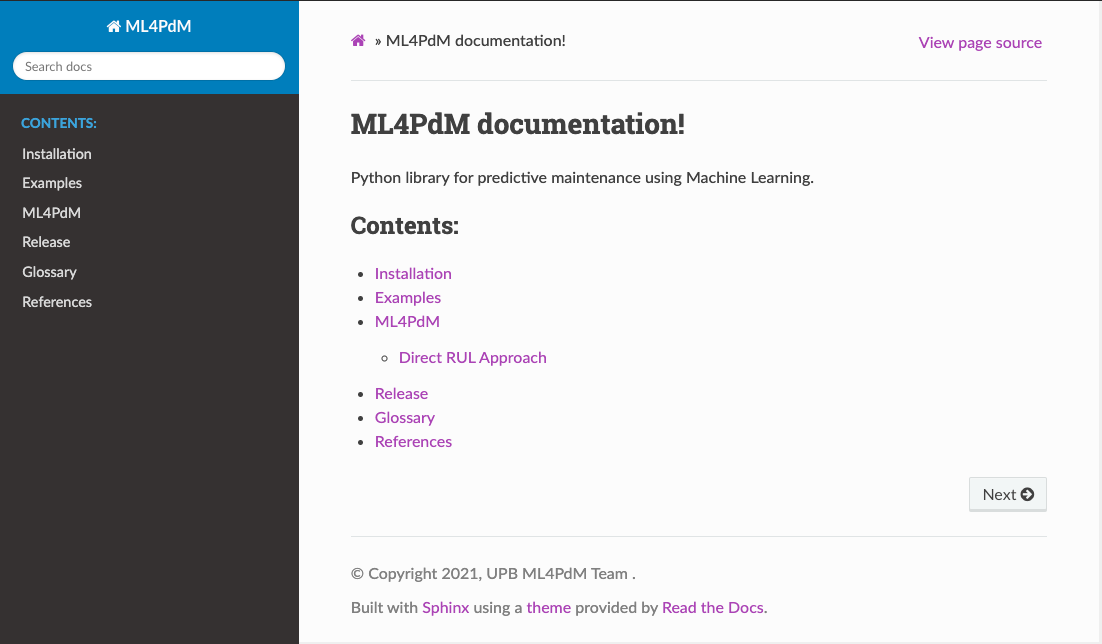
\includegraphics[width=12cm,height=6cm]{gfx/html.png}
	\caption{Example of HTML output of sphinx document generator for the planned sections.}
	\label{fig:html_output}
\end{figure}

\section{Git Strategy}
\vspace*{-10mm}\hfill{\fontfamily{phv}\normalsize\emph{Sanjay Gupta}}
\label{sec:quality_assurance:git}

In this section, we set the guidelines for the Git commit messages, versioning, Git structure, and branch merge. Git is a free and open-source distributed version control system that manages a project of any size. Having a good, git strategy will ease the work of DevOps which includes design, build, test, deploy, and maintenance. We are using the Gitflow workflow to achieve the task in a consistent and productive way. The Gitflow Workflow defines strict branching.

\subsection{Branches}
The Gitflow guides us to define what type of branches to set up and how to merge them together. Figure \ref{fig:git-workflow} demonstrates the working structure of Git workflow \cite{gitWorkflow}. The Git workflow consists of multiple branches of different types. For the ML4PdM project, we will define the three branches in the GitLab repository. The \textit{master} branch will be the default and stores the official release history in the repository. In \textit{master} branch will have only the tested and working implementations. The \textit{develop} branch will act as an integration branch for features. Each new feature should have its own branch, which is called the \textit{feature} branch. The \textit{feature} branch can be pushed or merged to develop and then master branch to make available that feature in a future release. The \textit{feature} branch isolates the task in-progress from the completed task. We are going to follow the \textbf{feature/<feature-name>} e.g.- feature/ci-pipeline as naming convention format for all \textit{feature} branches. We will not delete the \textit{feature} branches after the release So that we can apply bug fixes or hotfixes later on the same branch. The \textit{feature} branch use \textit{develop} as their parent branch. Once the feature is completed, it gets merged back into development. The \textit{master} should never interact directly with \textit{feature} branch. The \textit{feature} branch should be created from the latest \textit{develop} branch.
\begin{figure}[ht]
	\centering
	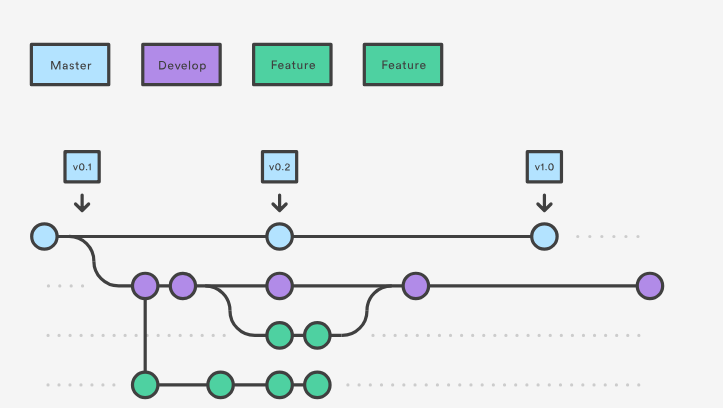
\includegraphics[width=\textwidth]{gfx/Git-Workflow.png}
	\captionsetup{justification=centering}
	\caption{Working of git workflow.}
	\label{fig:git-workflow}
\end{figure}

\subsection{Tags}
Tags are the process of assigning unique version numbers to unique states of the software packages. The tags are only created in the \textit{master} branch of the repository. For the ML4PdM project, we are going to follow the Semantic versioning tags for release packages. Semantic versioning is a standard convention for specifying compatibility using a three-part version number. We will follow the \textbf{Major.Minor.Patch} e.g.- v1.0.1, v1.0.0 format for our package release. The \textbf{Major} number is incremented when there are significant changes in functionality. The \textbf{Minor} number is incremented when only new features or major bug fixes have been added. The \textbf{Patch} number is incremented for minor changes and bug fixes.

\subsection{Commit Messages}
The content of the commit message outlining the change is just as important as the content of the change itself. For the ML4PdM project, we should use one of the below-listed commit constants in the subject line for the commit description.
\begin{enumerate}
	\item \textbf{[GEN]} - Use when code changes are related to general task like setup of document and etc.
	\item \textbf{[TFE]} - Use when code changes are related to Time Series Feature Extraction.
	\item \textbf{[HIE]} - Use when code changes are related to Health Index Estimation.
	\item \textbf{[RUL]} - Use when code changes are related to Remaining Useful Lifetime Estimation.
\end{enumerate}
While writing a commit message there are few important rules to keep in mind.
\begin{enumerate}
	\item Separate subject line from body with a blank line.
	\item Limit the subject line to 50 characters.
	\item Capitalize the subject line.
	\item Do not end the subject line with a period.
	\item Use the imperative mood in the subject line.
	\item Wrap the body at 72 characters.
	\item Can use the body to explain what and why vs how.
\end{enumerate}

\subsection{Merge}
The Merge command are designed to integrate changes from one branch into another branch. For ML4PdM project, We are using explicit merges (create new merge commit) strategy because it is simple, provide great traceability and context on the features being merged. The merge request should be reviewed by at least two people (Author and other team member) using GitLab approval feature in repository to maintain code quality. We are not going to squash and delete the source branch. Manual merge and rebase strictly not allowed in repository. The Figure \ref{fig:merge-request-template} show the merge request description template. Use the template, while requesting Merge Request (MR) to merge the proposed changes from one branch to another. In Added section, list or describe what are the new features added in proposed changes. In Changed section, list or describes the changes in the existing functionality. In Deprecated part, list or describe what are the feature will soon be removed. In Removed part, list or describe what features have been removed. In the Fixed part, list or describe what bugs fixes are.
\begin{figure}[ht]
	\centering
	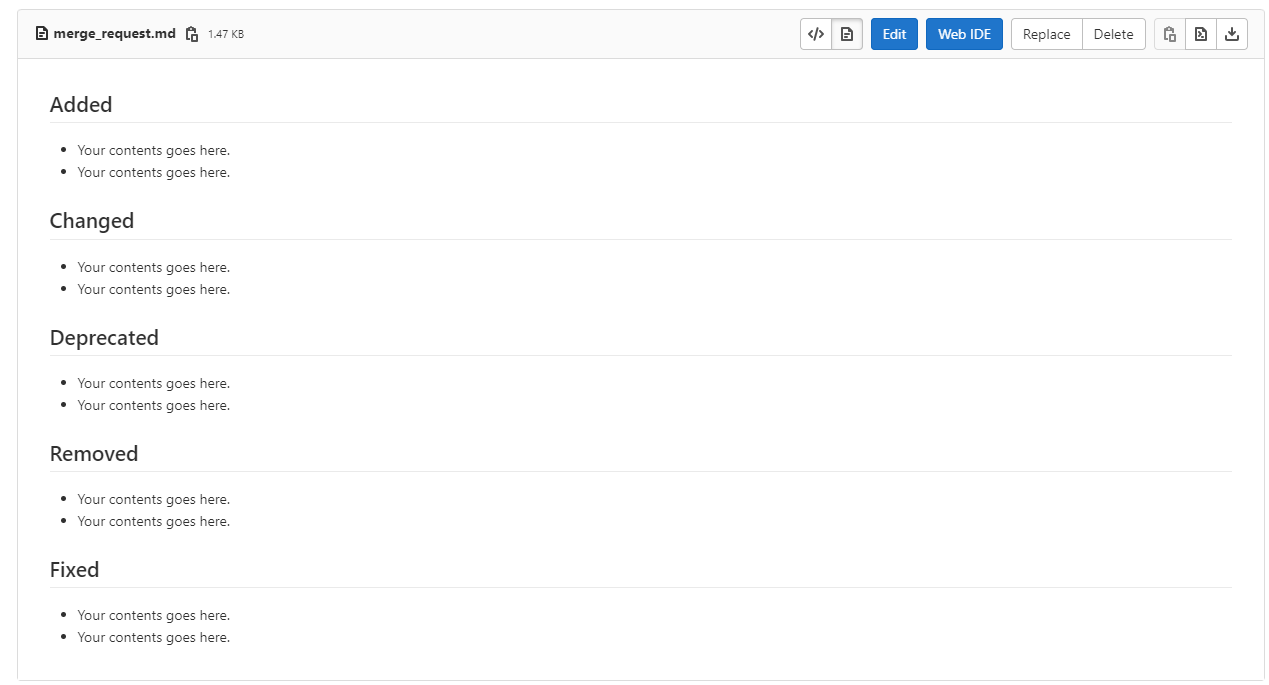
\includegraphics[width=\textwidth]{gfx/merge-request-template.PNG}
	\captionsetup{justification=centering}
	\caption{Structure of the Merge request template.}
	\label{fig:merge-request-template}
\end{figure}
